\chapter[Simulado 3]{Simulado}

\num{1} O número $\sqrt{8} + \sqrt{18}$ pode ser escrito como:

\begin{escolha}

  \item $\sqrt{26}$
  \item $2\sqrt{13}$
  \item $5\sqrt{2}$
  \item $\sqrt{10}$

\end{escolha}

\num{2} Em uma distribuidora de material para escritório, existem 100 
pilhas de resmas de papel A4, com cada pilha tendo 1 metro de altura. Cada 
resma contém 500 folhas de papel. O fornecedor informa na embalagem que a 
espessura de uma única folha é de 0,4 milímetros.

Quantas resmas existem na distribuidora?

\begin{escolha}

\item 2500

\item 2000

\item 1000

\item 500

\end{escolha}

\num{3} As operações entre dízimas periódicas podem ser realizadas 
por meio de frações que as representam. Se $x = 0,272727\ldots{}$ e 
$y = 0,5555\ldots{}$, qual o valor de x + y?

\begin{escolha}

\item $\frac{27}{99}$

\item $\frac{5}{9}$

\item $\frac{82}{99}$

\item $\frac{32}{108}$

\end{escolha}

\pagebreak
\num{4} Foi anunciada em uma loja de móveis usados a seguinte mesa de
escritório.

\begin{figure}[htpb!]
\centering
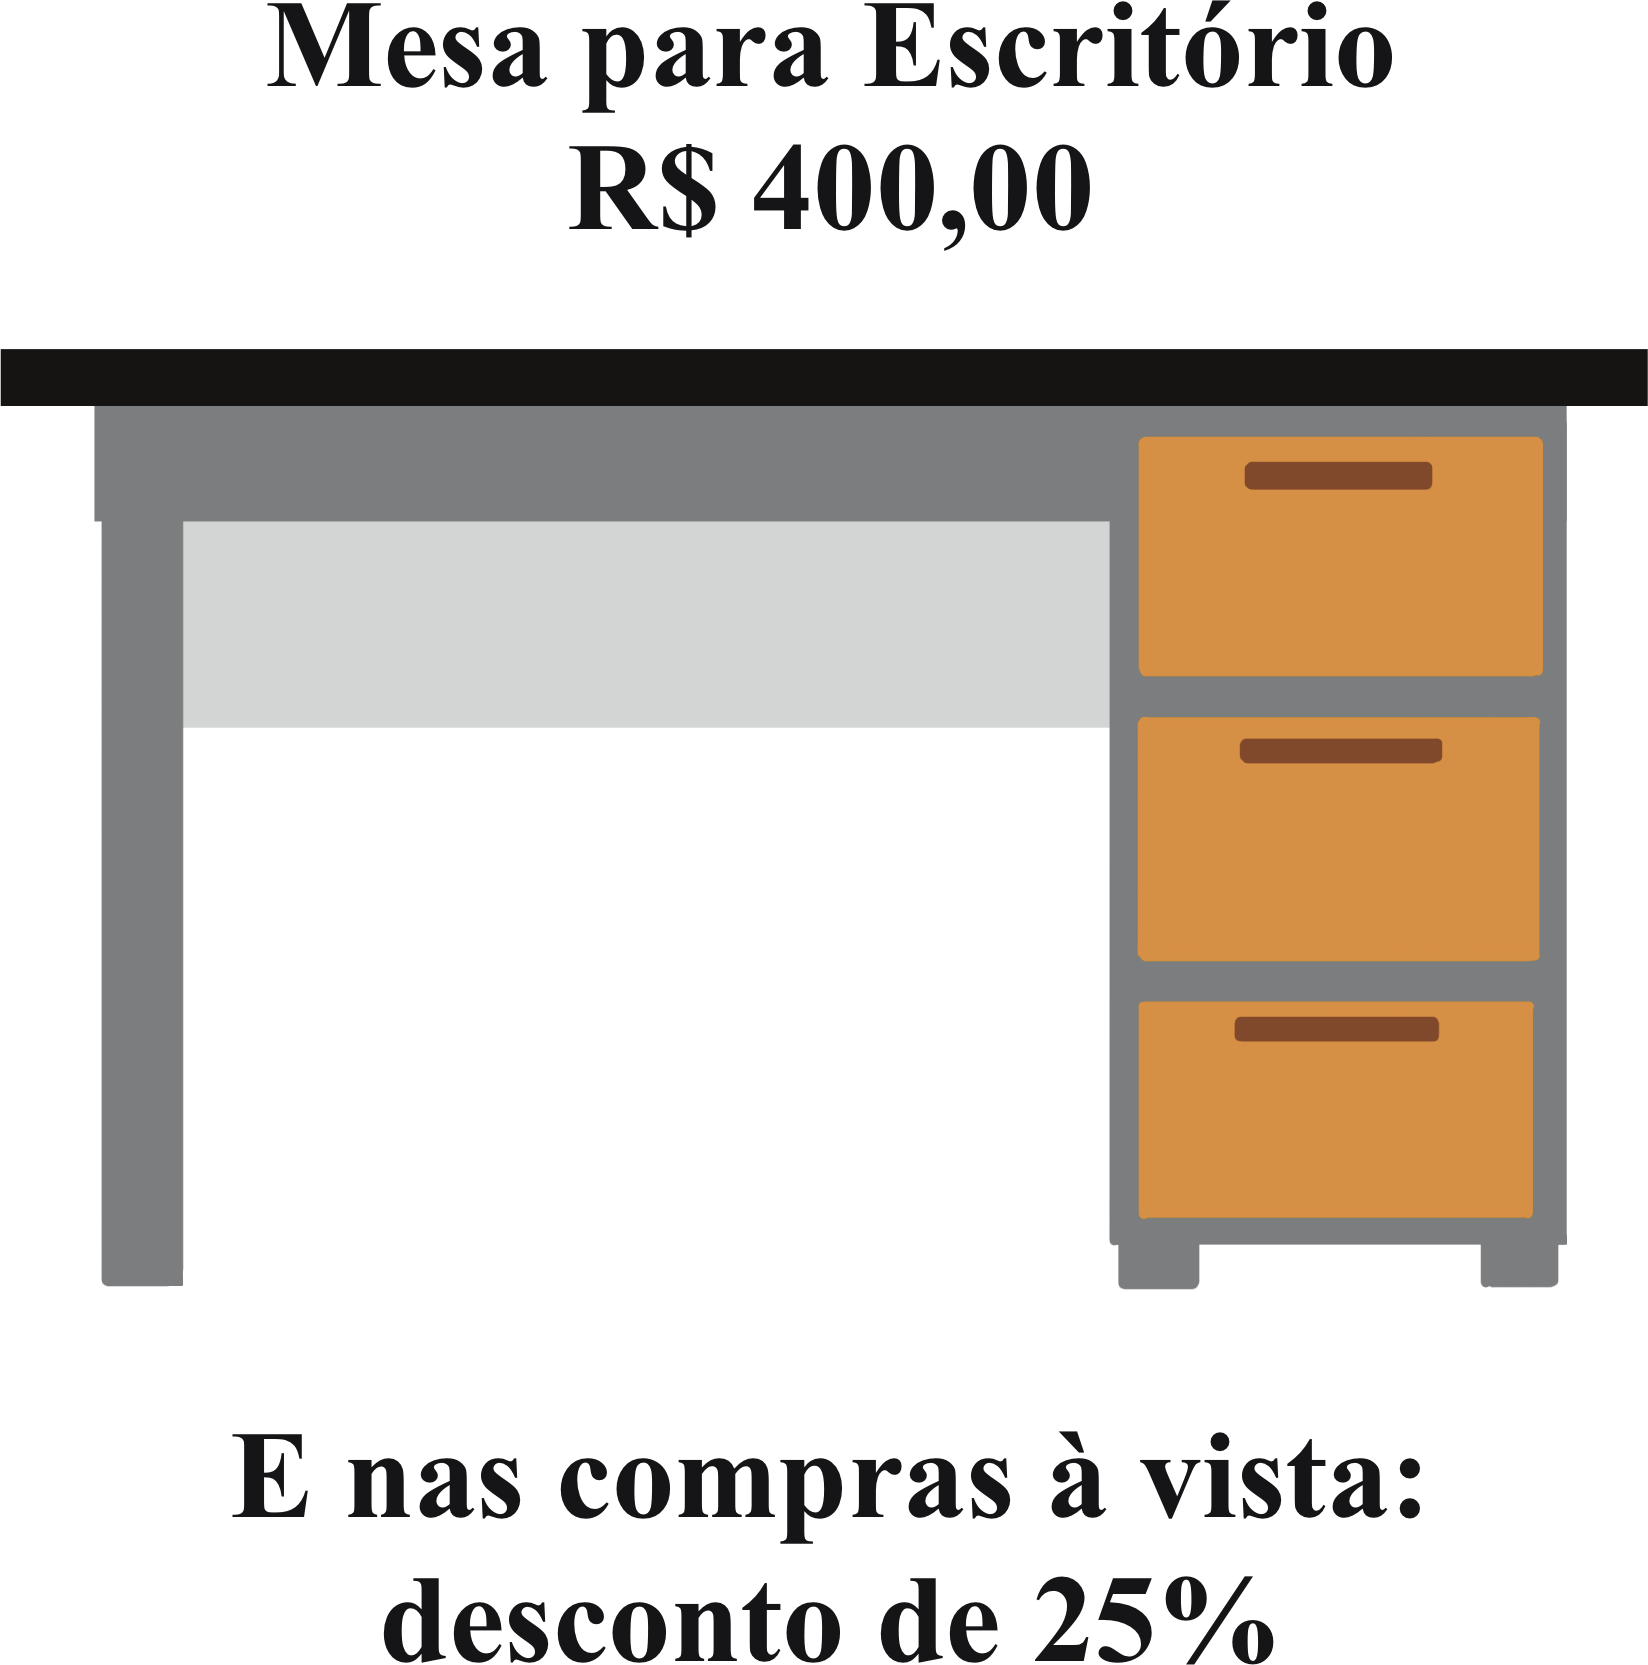
\includegraphics[width=.5\textwidth]{./ilustras-mat/Simulado_3-atividade_4.png}
\end{figure}


Qual será o valor da mesa pagamento à vista?

\begin{escolha}

\item R\$500,00

\item R\$350,00

\item R\$300,00

\item R\$100,00

\end{escolha}

\num{5} Observe a pesagem na balança abaixo, que está em equilíbrio. As
caixas de mesmo tamanho tem a mesma massa.

\begin{figure}[htpb!]
\centering
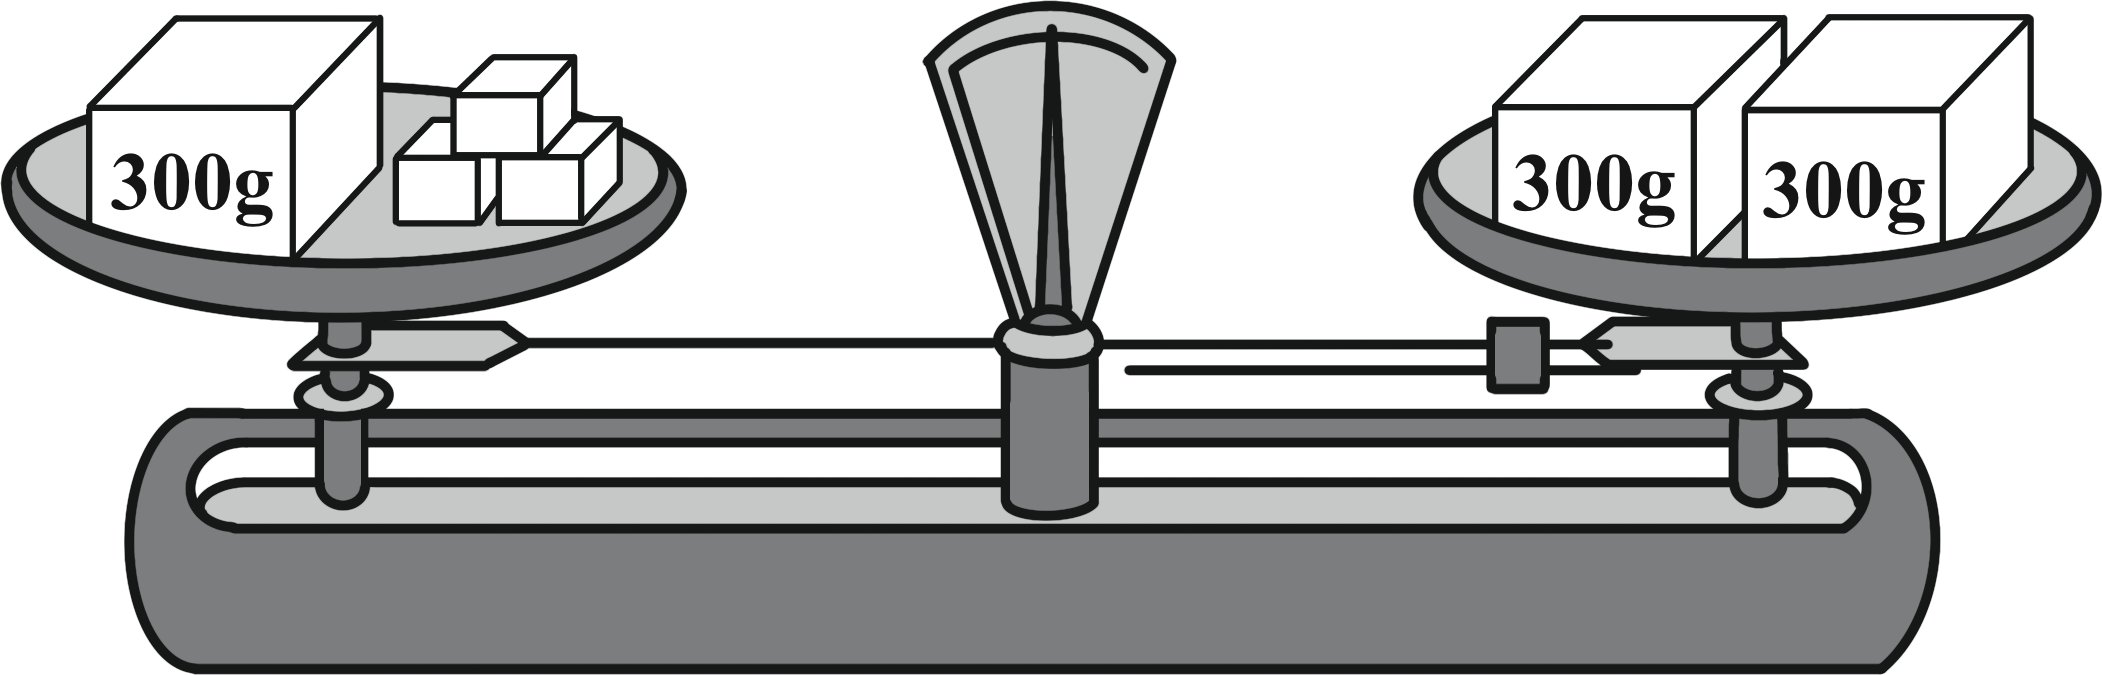
\includegraphics[width=.5\textwidth]{./ilustras-mat/Simulado_3-atividade_5.png}
\end{figure}

A massa da caixa pequena é

\begin{escolha}

  \item 50 g. 

  \item 100 g. 

  \item 150 g. 

  \item 300 g.

\end{escolha}

\pagebreak
\num{6} As variáveis x e y assumem valores conforme o quadro abaixo.

\begin{longtable}[]{@{}lllllll@{}}
\toprule
x & 5 & 6 & 7 & 8 & 9 & 10\tabularnewline
\midrule
\endhead
y & 17 & 21 & 25 & 29 & 33 & 37\tabularnewline
\bottomrule
\end{longtable}

A relação entre y e x é dada pela expressão:

\begin{escolha}
  
  \item $y = 4x + 1$. 
  
  \item $y = 2x + 2$ 
  
  \item $y = 4x - 3$ 
  
  \item $y = 3x + 2$

\end{escolha}

\num{7} Os valores referentes às duas raízes da equação $x² + 2x - 24
= 0$ estão no intervalo

\begin{escolha}

  \item de 4 até 6. 

  \item de --7 até 5. 

  \item de --5 até 7. 

  \item de --6 até 2.

\end{escolha}

\num{8} Josias é zelador em um condomínio, por isso contratou um jardineiro
para cortar o gramado. Para fazer o serviço em uma área de 
40 m\textsuperscript{2}, foram necessários 80 minutos. O gramado está
representado pela figura, indicando os espaços onde o trabalho já foi
realizado e onde o gramado ainda deve ser aparado.

\begin{figure}[htpb!]
\centering
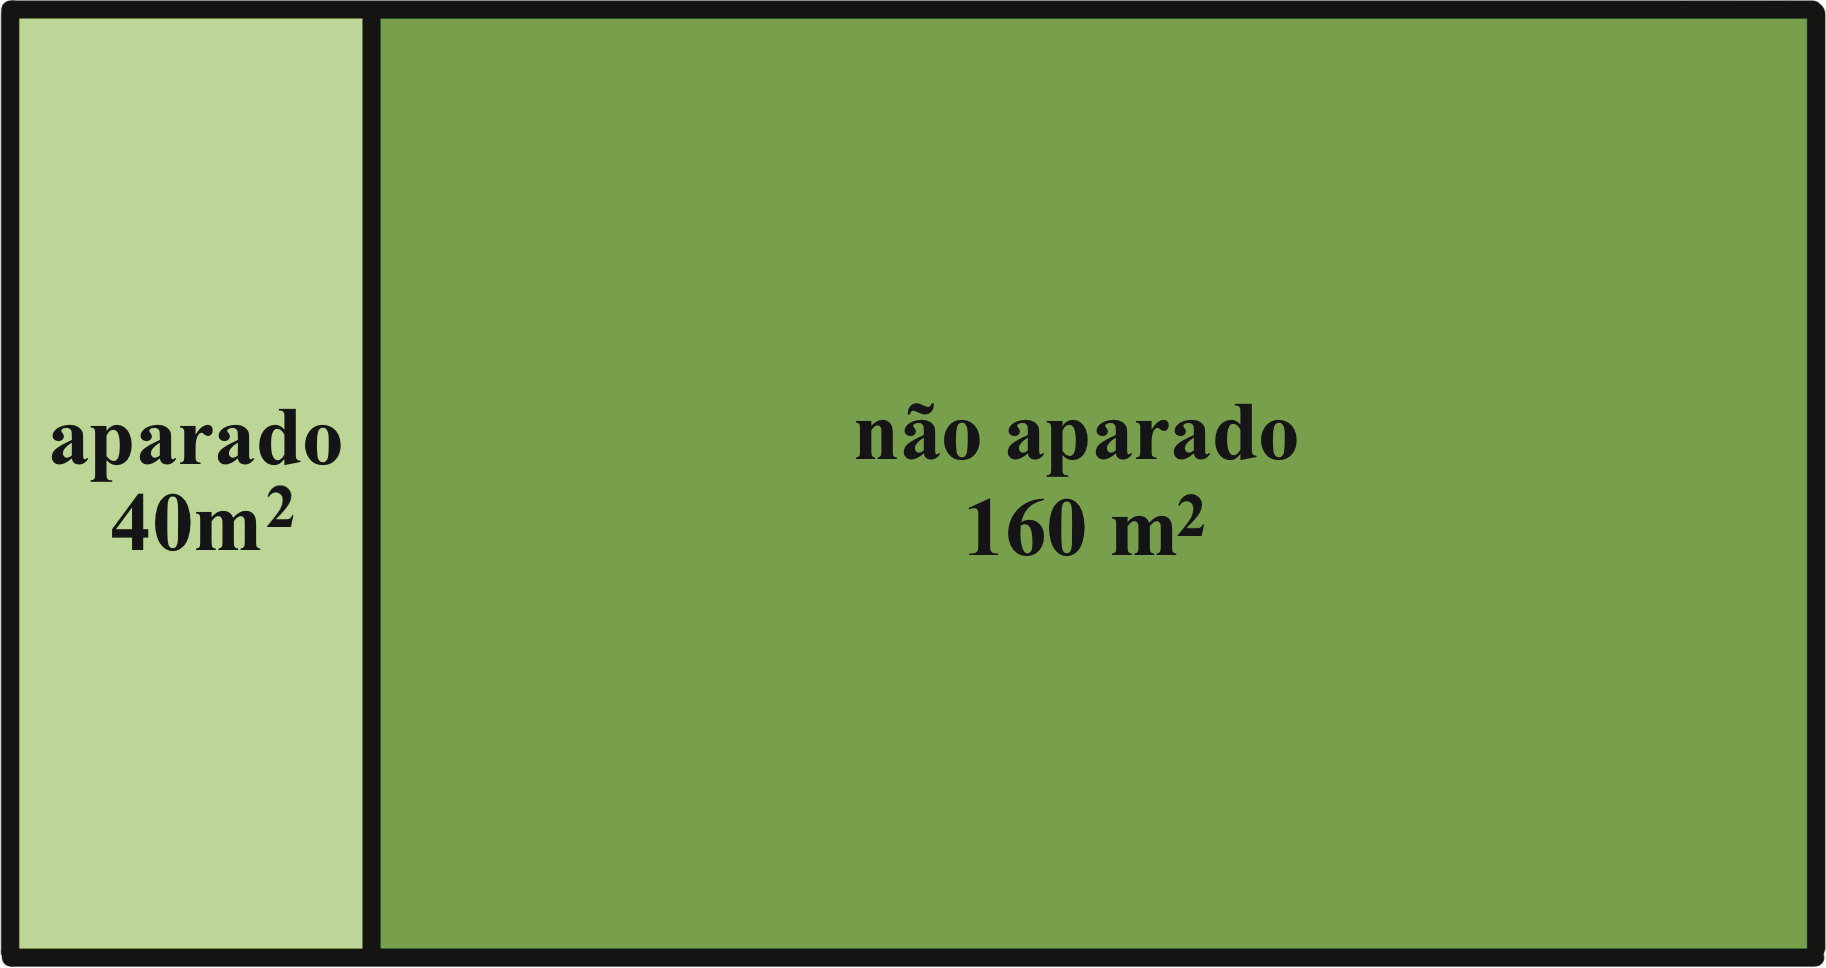
\includegraphics[width=.9\textwidth]{./ilustras-mat/Simulado_3-atividade_8.png}
\end{figure}

\pagebreak
Considerando que o jardineiro mantenha o mesmo ritmo de trabalho no
restante do gramado, qual o tempo, em minutos, previsto para que o
jardineiro conclua o serviço de corte do gramado?

\begin{escolha}

  \item 320

  \item 200

  \item 120

  \item 100

\end{escolha}

\num{9} Jorge fez um estudo em laboratório acompanhando a população de um
determinado vírus. Ele montou a tabela a seguir.

\begin{longtable}[]{@{}ll@{}}
\toprule
Tempo em minutos & Quantidade\tabularnewline
\midrule
\endhead
1 & 1\tabularnewline
2 & 5\tabularnewline
3 & 9\tabularnewline
4 & 13\tabularnewline
5 & 17\tabularnewline
\bottomrule
\end{longtable}

Supondo-se que o ritmo de crescimento dessa população tenha continuado a
obedecer a essa mesma lei, o número de vírus, ao final de 30 minutos,
era:

\begin{escolha}

  \item 102

  \item 117

  \item 197

  \item 200

\end{escolha}

\pagebreak
\num{10} Na figura abaixo, temos um quadrado AEDF, $\bar{AC} = 8$ e $\bar{AB} = 12$.

\begin{figure}[htpb!]
\centering
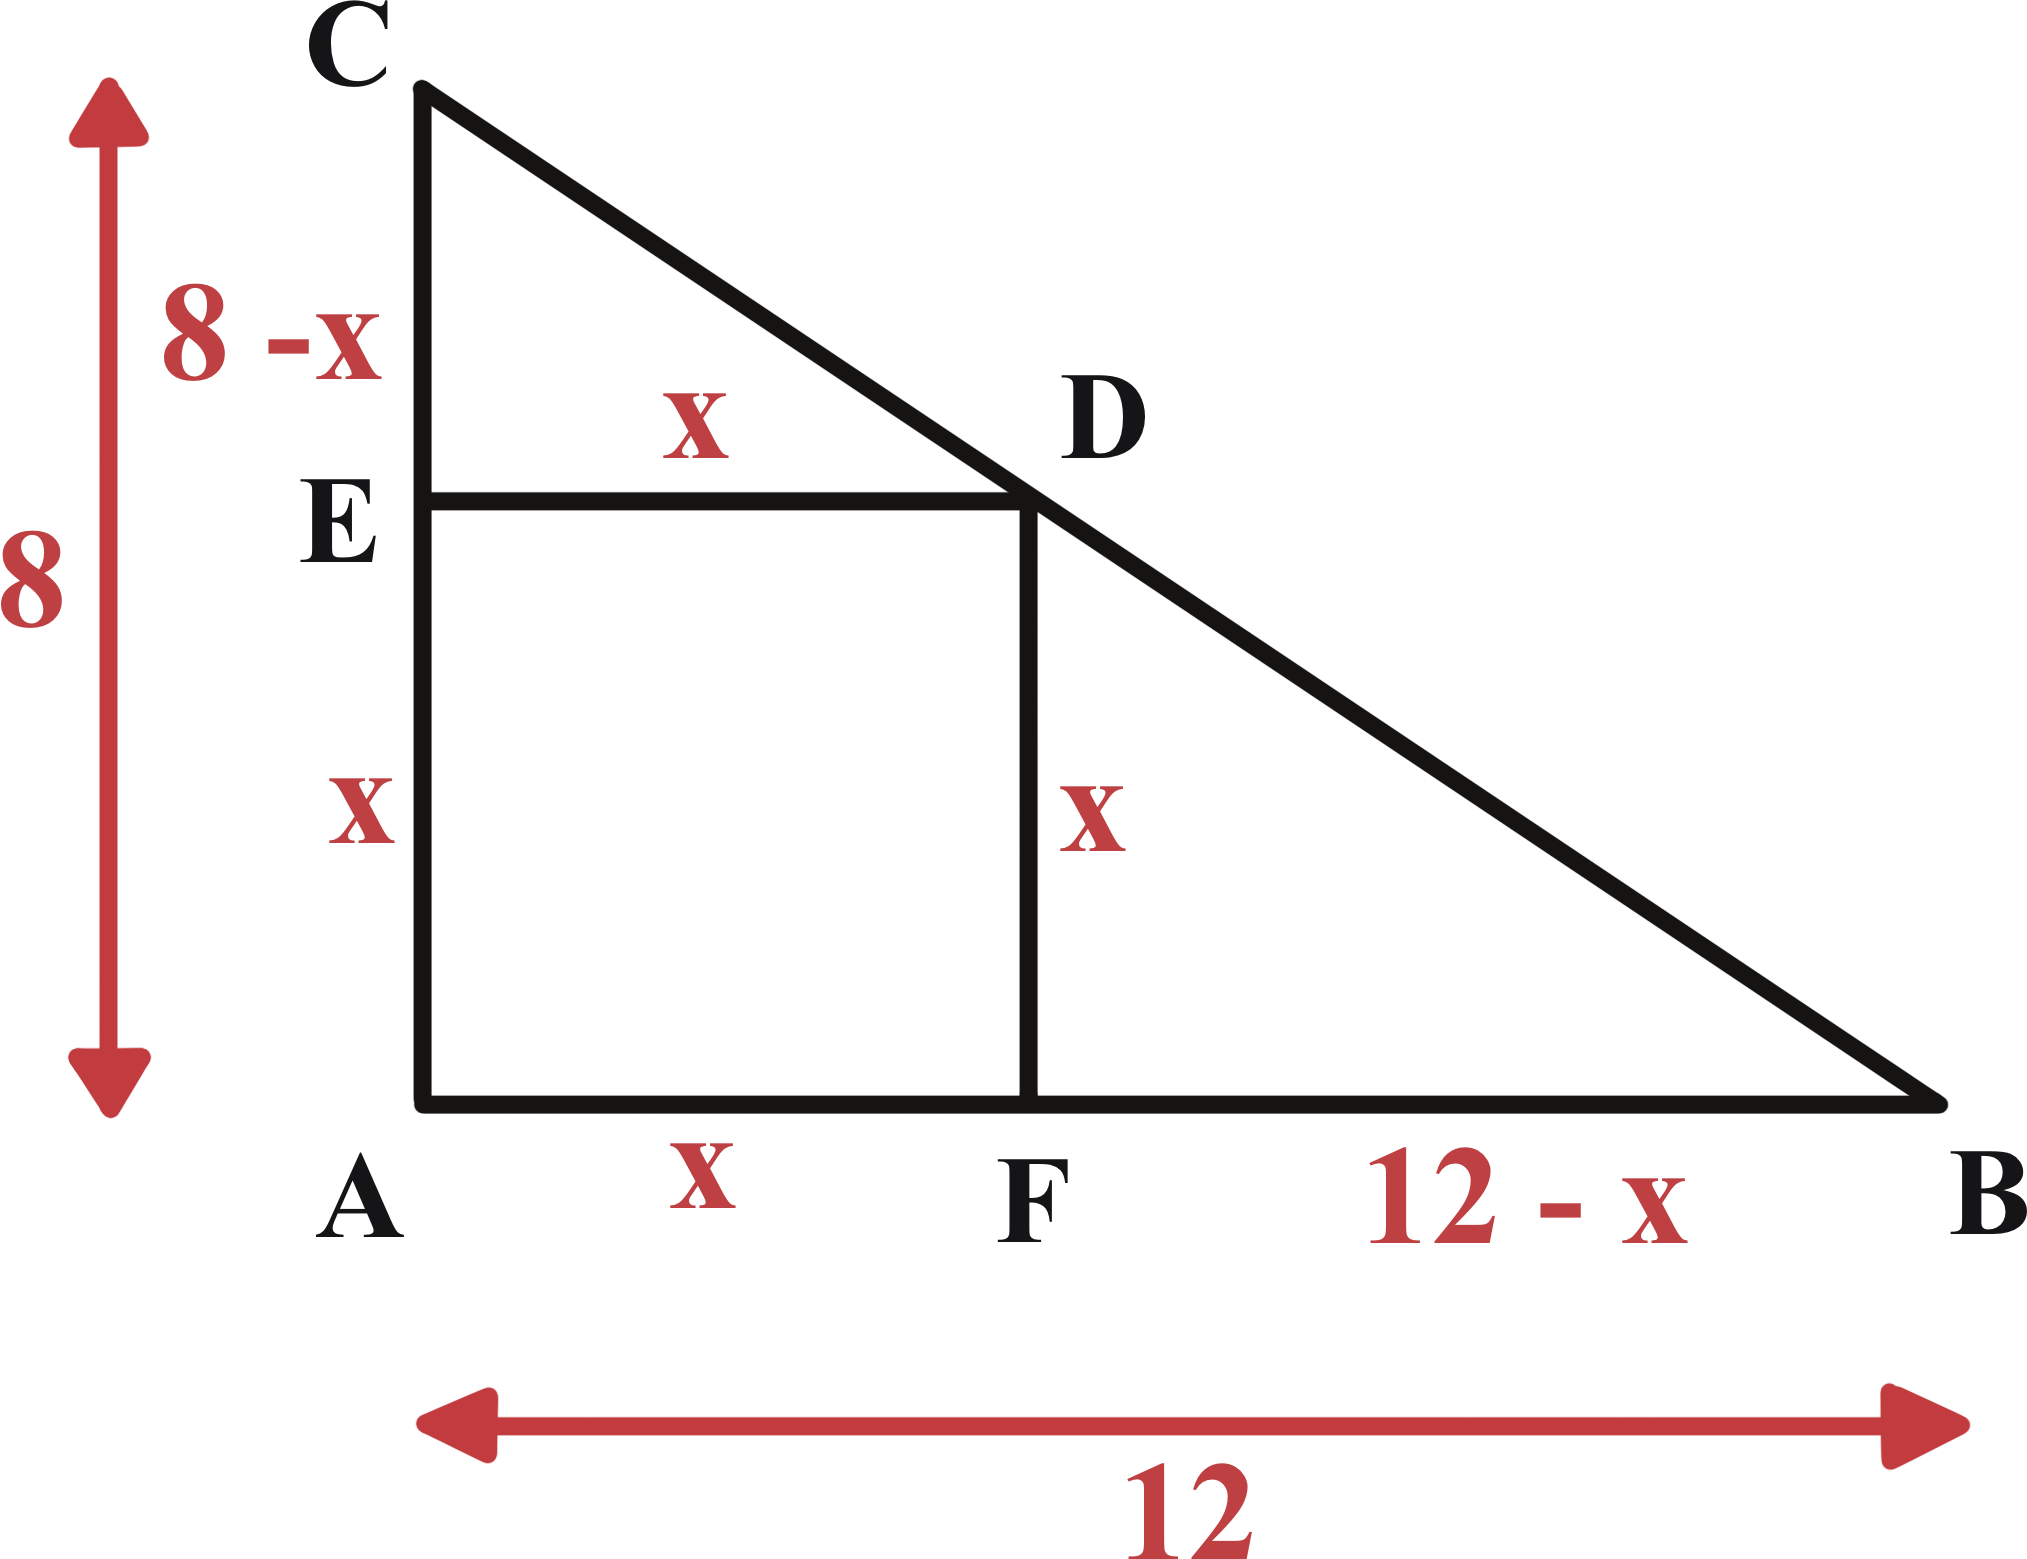
\includegraphics[width=.5\textwidth]{./ilustras-mat/Simulado_3-atividade_10_resposta.png}
\end{figure}

Qual é área do quadrado?

\begin{escolha}

  \item 5,76

  \item 4,8

  \item 20

  \item 23,04

\end{escolha}


\num{11} Em um triângulo retângulo, a hipotenusa mede 13 cm e um
dos catetos tem 5 cm.

Qual a medida do outro cateto?

\begin{escolha}

  \item 12

  \item 11

  \item 10

  \item 8

\end{escolha}

\pagebreak
\num{12} Os gráficos a seguir mostram, em milhões de reais, o total do
valor das vendas que uma empresa realizou em cada mês, nos anos de 2021
e 2022.

\begin{figure}[htpb!]
\centering
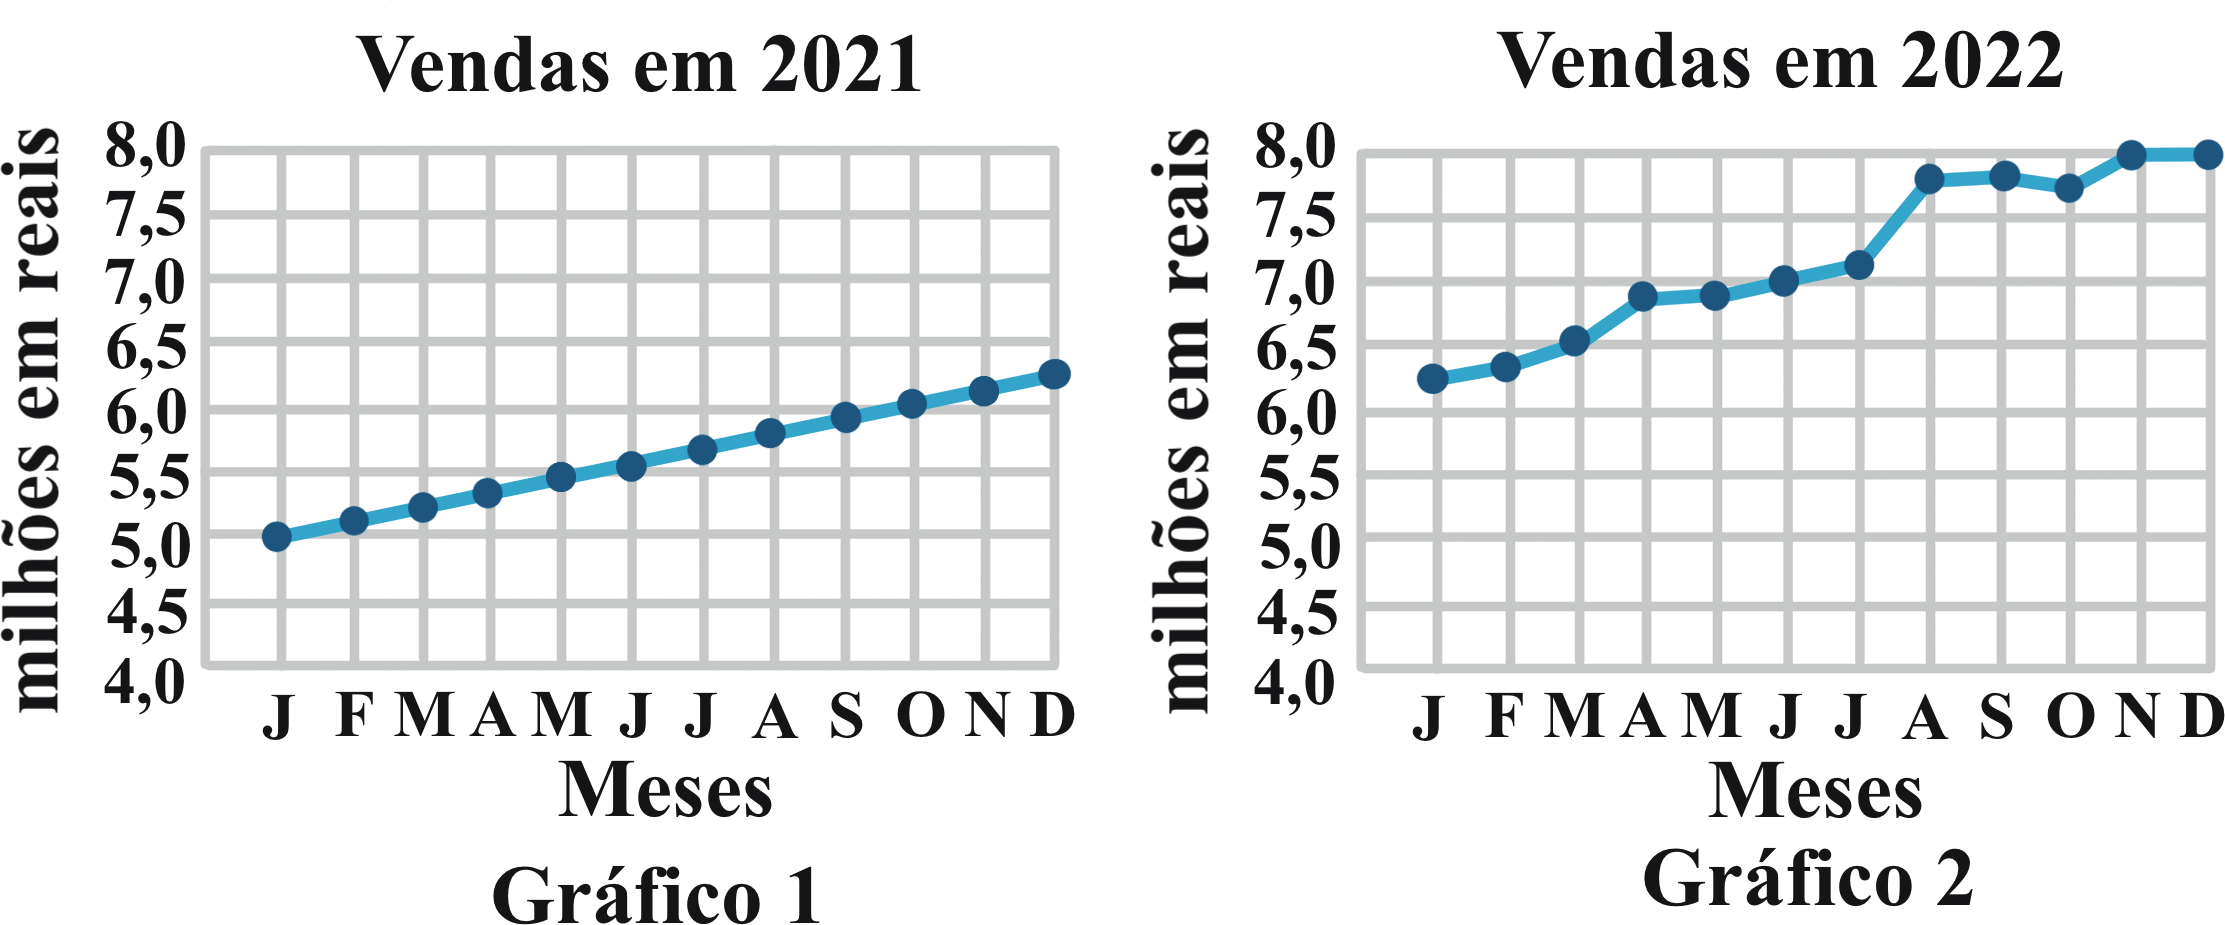
\includegraphics[width=\textwidth]{./ilustras-mat/Simulado_3-atividade_12.png}
\end{figure}

As vendas em 2022 foram bem melhores que as de 2021, mas observando o
gráfico pode-se afirmar que:

\begin{escolha}

  \item em 2021 houve oscilações bruscas nas vendas mensais.

  \item houve queda brusca das vendas de julho para agosto de 2022.

  \item houve queda nas vendas do mês de setembro para outubro em 2022.

  \item o maior aumento ocorreu entre novembro para dezembro de 2022.

\end{escolha}

\num{13} Um dado foi lançado 100 vezes. A tabela a seguir mostra os seis
resultados possíveis e as suas respectivas frequências de ocorrências:

\begin{center}
\begin{tabular}{|c|c|c|c|c|c|c|}
  \hline \textbf{Resultado} & 1 & 2 & 3 & 4 & 5 & 6 \\ \hline
\textbf{Frequência} & 14 & 21 & 15 & 12 & 18 & 20 \\ \hline
\end{tabular}
\end{center}

Qual a moda dos resultados?

\begin{escolha}

  \item 2

  \item 3

  \item 4

  \item 5

\end{escolha}

\pagebreak
\num{14} Marcos comprou uma TV no valor de R\$ 4.500,00. Ele optou por dar
30\% de entrada e o restante foi negociado em 5 parcelas sem juros.

Qual o valor da parcela?

\begin{escolha}
  \item R\$ 135,00

  \item R\$ 315,00

  \item R\$ 530,00

  \item R\$ 630,00
\end{escolha}

\num{15} Considere o lançamento simultâneo de dois dados
distinguíveis e não viciados, isto é, em cada dado, a chance de se obter
qualquer um dos resultados $(1, 2, 3, 4, 5, 6)$ é a mesma. A probabilidade
de que a soma dos resultados seja 7 é:

\begin{escolha}

  \item $\frac{5}{36}$

  \item $\frac{1}{2}$

  \item $\frac{1}{3}$

  \item $\frac{1}{6}$

\end{escolha}

\num{16}  Leia o texto a seguir:

\begin{quote}
Na condição de cultura urbana, o hip hop surgiu na periferia de Nova
York, entre as comunidades caribenhas, afro-americanas e
latino-americanas na década de 1970. O contexto social era de violência
e criminalidade nesses bairros, e a única forma de lazer possível para
os jovens era nas ruas. Encontraram na música, poesia, dança e na
pintura uma forma de manifestação de sua realidade e contestação.

\fonte{Governo do Estado do Ceará. Iniciação ao Hip hop desperta
interesse dos adolescentes no Projeto ``Danças Urbanas''. Disponível em:
https://www.seas.ce.gov.br/2021/08/05/iniciacao-ao-hip-hop-desperta-interesse-dos-adolescentes-no-projeto-dancas-urbanas/\#:\textasciitilde{}:text=Origem\%20do\%20Hip\%20Hop,os\%20jovens\%20era\%20nas\%20ruas.
Acesso em: 22 fev. 2023.}
\end{quote}

Considerando as informações da reportagem, é possível afirmar que o
hip hop surgiu com o objetivo de

\begin{escolha}
\item incentivar a prática esportiva em espaços abertos.

\item estimular o empreendedorismo social.

\item reduzir a violência na cidade por meio da arte.

\item contestar a realidade social de maneira pacifica.
\end{escolha}

\pagebreak
\num{17}  Leia o texto a seguir.

\begin{quote}
Segundo o Blog da Saúde, a vigorexia é um tipo de transtorno dismorfóbico
-- de distorção da autoimagem {[}...{]}

Desse modo, a vigorexia é uma doença psicológica caracterizada pela
insatisfação constante com o corpo {[}...{]}

\fonte{Ministério da Saúde. Precisamos falar do excesso de atividade física: você sabe o que é
vigorexia? Disponível em:
https://www.gov.br/saude/pt-br/assuntos/saude-brasil/eu-quero-me-exercitar/noticias/2021/precisamos-falar-do-excesso-de-atividade-fisica-voce-sabe-o-que-e-vigorexia.
Acesso em: 12 abr. 2023.}
\end{quote}

A prática mais comum da pessoa acometida pela vigorexia é a

\begin{escolha}
\item obsessão pela alimentação saudável.

\item prática de exercícios físicos em excesso.

\item indução do vômito após uma refeição.

\item ingestão de pequenas quantidades de alimentos.
\end{escolha}

\num{18}  Leia o texto a seguir

\begin{quote}
\textit{Doping} refere-se ao uso de substâncias naturais ou sintéticas
visando a melhora do desempenho dos atletas em competições. Este objetivo 
é ilícito e por isso são feitos testes de \textit{doping} durante competições.

\fonte{Secretaria da Educação. Doping. Disponível em:
http://www.ciencias.seed.pr.gov.br/modules/galeria/detalhe.php?foto=1845\&evento=1.
Acesso em: 22 fev. 2023.}
\end{quote}

Considerando a definição proposta no texto, pode-se inferir que os atletas
que praticam \textit{doping} são aqueles que

\begin{escolha}
\item evitam o uso de substâncias ilegais.

\item usam medicamentos proibidos para ganhar as competições.

\item pretendem recuperar-se de lesões.

\item aplicam os anabolizantes para cuidar da saúde.
\end{escolha}

\num{19}
\begin{quote}
  O nome, que vem do grego~\emph{atomos}, significa algo como "indivisível". Os
  físicos, porém, tempos depois, já entendem que os átomos não são sólidos como pequenas
  esferas, mas uma espécie de sistema planetário em miniatura. São constituídos por três partes principais: prótons, nêutrons e
  elétrons -- prótons e nêutrons unidos no centro, como um ``sol'' (núcleo). Elétrons, por sua vez, orbitando esse núcleo, assim como os planetas. 

\fonte{Fonte de pesquisa: BBC News Brasil.  21/01/2016. Disponível em:
https://www.bbc.com/portuguese/noticias/2016/01/160113\_vert\_earth\_como\_sabemos\_que\_atomos\_existem\_rw.
Acesso em: 24 fev. 2023.}
\end{quote}

\pagebreak
Sabendo que os elétrons podem se movimentar independentemente de seus
átomos, escolha a alternativa que justifica um possível experimento para
provar essa movimentação dos elétrons.

\begin{escolha}
\item
  Submeter os elétrons a um processo de liofilização para observar se havia uma repulsão de cargas.
\item
  Colocar os elétrons sobre feixes de luz superpotentes para que fosse
  possível observar sua movimentação.
\item
  Ionizar os átomos, doando cargas negativas para repelirem os elétrons e
  observar sua movimentação.
\item
  Centrifugar os elétrons, já que nesse processo seriam doadas cargas
  positivas, e observar se há movimentação.
\end{escolha}

\num{20}
\begin{quote}
Com o objetivo de preservar a biodiversidade e garantir o menor
impacto ambiental possível em projetos de infraestrutura de
transportes, Ministério dos Transportes e Instituto Brasileiro do Meio
Ambiente e dos Recursos Naturais Renováveis (Ibama) decidiram
fortalecer a parceria entre os dois órgãos do Governo Federal. 
Nesta
quinta-feira (23), o ministro dos Transportes, Renan Filho, e o
presidente do Instituto Brasileiro do Meio Ambiente e dos Recursos
Naturais Renováveis (Ibama), Rodrigo Agostinho, reuniram-se para
tratar de projetos em rodovias onde há grande riqueza de fauna e
flora, incluindo espécies ameaçadas de extinção, os quais necessitam
da junção de esforços visando à preservação ambiental. [...]

\fonte{Governo Federal do Brasil. Parceria vai fortalecer preservação de fauna e flora nas imediações de rodovias. Disponível em:
https://www.gov.br/infraestrutura/pt-br/assuntos/noticias/2023/02/parceria-vai-fortalecer-preservacao-de-fauna-e-flora-nas-imediacoes-de-rodovias.
Acesso em: 25 fev. 2023.}
\end{quote}

Uma possível medida que visa a conciliar o avanço da infraestrutura do país com a proteção ambiental é

\begin{escolha}
\item
  Construir corredores ecológicos entre as vias para que os animais
  possam atravessar entre os ambientes em segurança.
\item
  Investir na locomoção por vias aquáticas e aéreas para evitar a
  construção de pistas e a degradação ambiental.
\item
  Isolar cidades e comunidades que vivem em regiões de alta
  biodiversidade, evitando a degradação ambiental.
\item
  Cobrar taxas de circulação para quem for circular por vias que se
  localizem em regiões onde há presença de animais silvestres.
\end{escolha}

\pagebreak
\num{21}
  Na antiguidade o eclipse solar era considerado algo místico. Na Grécia
  antiga, por exemplo, o eclipse solar era sinônimo da ira dos Deuses.
  Com o avanço da ciência foi possível identificar o que de fato é um
  eclipse solar e como ele acontece.

\fonte{Texto autoral.}

Identifique, a partir das alternativas a seguir, aquela que explica
corretamente como ocorre um eclipse solar.

\begin{escolha}
\item
  Um eclipse solar ocorre quando o Sol se posiciona entra a Terra e a Lua.
\item
  Um eclipse solar ocorre quando a Lua se posiciona entra a Terra e o Sol.
\item
  Um eclipse solar ocorre quando Marte e a Lua passam entre o Sol e a Terra.
\item
  Um eclipse solar ocorre quando a Terra fica entre o Sol e a Lua.
\end{escolha}

